%versi 2 (8-10-2016) 
\chapter{Pendahuluan}
\label{chap:intro}
   
\section{Latar Belakang}
\label{sec:label}
Ujian menjadi salah satu syarat yang mutlak untuk memenuhi komponen penilaian
suatu mata kuliah. Salah satu bentuk ujian tersebut dilakukan secara praktik.
Ujian praktik ini dilaksanakan pada lab komputasi dengan bantuan aplikasi. Pihak
yang bertanggung jawab untuk mempersiapkan ruangan dan sistem adalah
\textit{System Administrator} atau Admin. Peserta akan diberi soal ujian melalui
sistem yang berjalan di lab sesuai prosedur dan aturan yang berlaku.

Ujian pada Lab Komputasi dilakukan dengan bantuan perangkat lunak. Perangkat
lunak tersebut membantu mengatur berbagai kebutuhan seperti pengumpulan jawaban,
pengacakan daftar peserta, serta pengarsipan berkas jawaban. Perangkat lunak
yang saat ini digunakan bernama Oxam (Gambar \ref{fig:ss-Oxam}). Oxam bekerja
dengan meminta parameter berupa kode matakuliah, tipe ujian, jurusan, jam mulai
ujian, daftar peserta, \textit{slot} tempat duduk yang dapat digunakan, dan
daftar nama berkas yang akan dikumpulkan. Perangkat lunak Oxam akan secara
otomatis membuatkan daftar tempat duduk peserta yang sudah teracak, dan
membuatkan \textit{script} untuk menyalin berkas ujian ke komputer peserta.

\begin{figure}
    \centering
    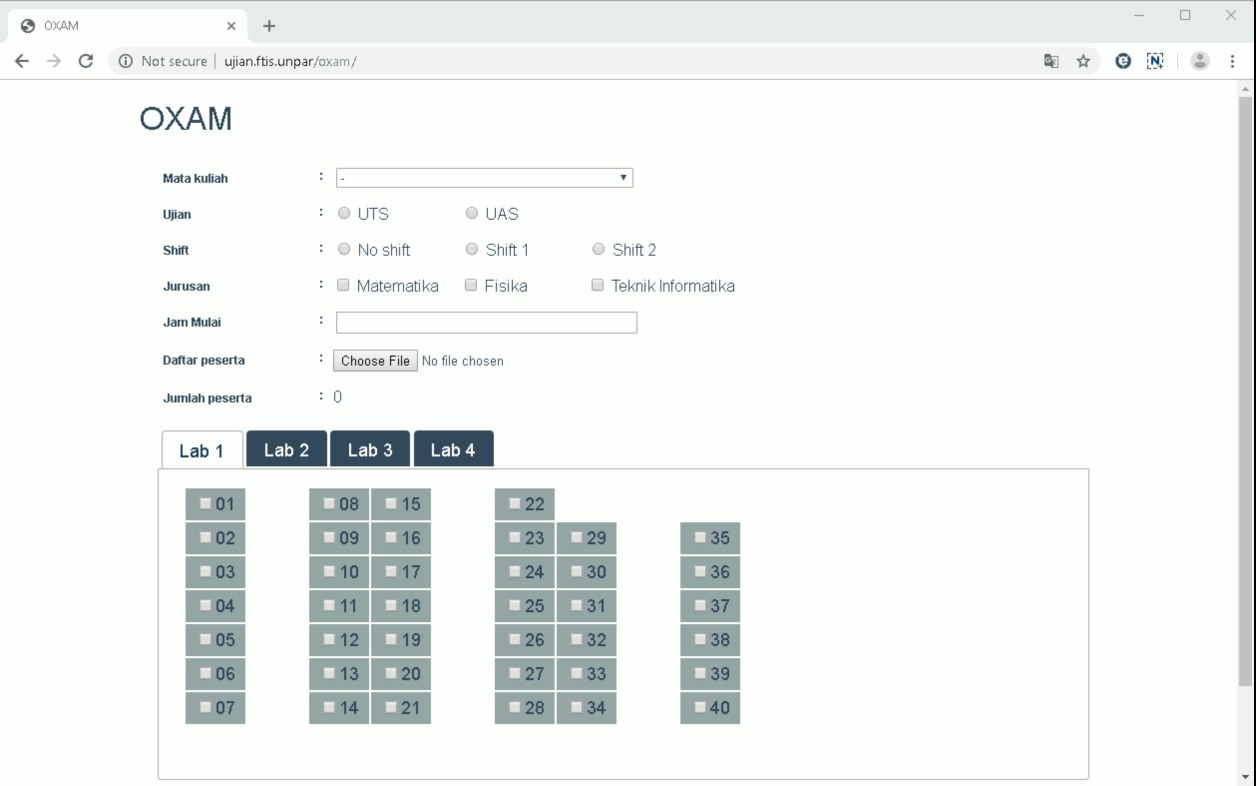
\includegraphics[width=0.7\paperwidth]{Gambar/ss-oxam.png}
    \caption{Tampilan cuplikan layar dari Oxam, aplikasi manajemen ujian di Lab Komputasi.}
    \label{fig:ss-Oxam}
\end{figure}

Namun fitur yang terbatas membuat Oxam menjadi tidak efektif untuk menyelesaikan
insiden-insiden khusus. Salah satu masalah yang sering dihadapi adalah
perpindahan posisi peserta ke meja lain saat masalah terjadi. Admin harus
mengubah secara manual entri pada database yang bersangkutan, lalu memindahkan
berkas ujian tersebut secara manual ke posisi yang baru. Perubahan NPM (Nomor
Pokok Mahasiswa) untuk angkatan 2018 dan seterusnya membuat sistem Oxam yang
lama tidak dapat digunakan tanpa harus mengubah NPM tersebut ke bentuk yang
lama, lihat Tabel \ref{tab:table-npm}. 

\begin{table}[H]
    \centering
    \def\arraystretch{2}
    \begin{tabular}{|c|c|}
        \hline
        \textbf{NPM Lama} & \textbf{NPM Baru} \\
        \hline
        201673\textbf{0011} & 6181601\textbf{011} \\
        \hline
        \multicolumn{2}{|c|}{\textbf{username}} \\
        \hline
        \multicolumn{2}{|c|}{i16\textbf{011}} \\
        \hline
    \end{tabular}
    \caption{NPM lama, baru dan username yang mahasiswa gunakan untuk login.}
    \label{tab:table-npm}
\end{table}

NPM lama memiliki empat komponen besar yang digunakan untuk mengidentifikasi
jenis mahasiswa (Tabel \ref{tab:table-npm}, kolom NPM Lama). 
\begin{itemize}
    \item Empat karakter pertama pada NPM adalah informasi tahun mahasiswa
    tersebut memulai kuliah. Pada contoh tampak angka 2016, yang berarti
    mahasiswa tersebut memulai perkuliahannya pada tahun 2016 (angkatan 2016). 
    
    \item Dua karakter berikutnya menandakan jurusan (dan fakultas) mahasiswa
    tersebut belajar. Pada contoh tampak angka 73 yang menandakan bahwa
    mahasiswa tersebut belajar pada Fakultas Teknologi Informasi dan Sains (7),
    dan berada pada jurusan Informatika (73). 
    
    \item Satu karakter berikutnya menandakan program yang diambil oleh
    mahasiswa tersebut. Angka 0 menunjukkan bahwa mahasiswa tersebut mengikuti
    program Sarjana, seperti pada tabel contoh. Angka 1 menandakan mahasiswa
    tersebut mengambil program pascasarjana dan angka 2 menunjukkan program
    doktoral. 
    
    \item Tiga angka berikutnya yang menjadi komponen terakhir dari NPM lama ini
    adalah nomor urut mahasiswa tersebut. Dengan spesifikasi berikut,
    berdasarkan tabel contoh, mahasiswa dengan NPM 2016730011 adalah mahasiswa
    angkatan 2016, mengikuti program sarjana informatika pada Fakultas Teknologi
    Informasi dan Sains dengan nomor urut 11.
\end{itemize}

NPM baru ini dibuat pada tahun 2018, dan memiliki struktur yang jauh berbeda
dari NPM lama. Format NPM tersebut didefinisikan sebagai berikut:

\begin{itemize}
    \item Angka pertama menandakan program jenjang yang diambil oleh mahasiswa
    tersebut. Angka 5 untuk diploma, 6 untuk sarjana, 8 pascasarjana dan 9 untuk
    doktoral. 

    \item Dua digit angka berikutnya menunjukkan program studi yang diambil oleh
    mahasiswa tersebut, pada contoh 18 berarti Informatika. 
    
    \item Dua digit berikutnya menunjukan angka tahun mulai perkuliahan
    (angkatan) dalam format representasi tahun dengan dua digit. Pada contoh
    tampak angka 16 yang berarti mahasiswa tersebut adalah angkatan 2016. 
    
    \item Dua digit berikutnya menginformasikan jenis mahasiswa. Pada contoh
    tampak angka 01 yang menandakan bahwa mahasiswa tersebut berjenis reguler.
    
    \item Tiga digit terakhir menginformasikan nomor urut mahasiswa tersebut.
\end{itemize}

Pada tabel \ref{tab:table-npm} terdapat kolom username yang digunakan untuk
menstandarisasi NPM tersebut. Informasi username ini nantinya dimanfaatkan untuk
mengintegrasi berbagai macam sistem yang membutuhkan informasi mahasiswa. Digit
pertama pada username menginformasikan jurusan mahasiswa tersebut. Huruf i
menginformasikan mahasiswa tersebut adalah mahasiswa jurusan Informatika, huruf
m untuk matematika, dan huruf f untuk fisika. Dua digit berikutnya
menginformasikan tahun angkatan mahasiswa tersebut dalam bentuk representasi
tahun dalam dua digit. Pada contoh tampak angka 16, yang menandakan bahwa
username ini adalah milik mahasiswa angkatam 2016. Tiga digit terakhir
berikutnya menginformasikan nomor urut mahasiswa tersebut.

Karena sistem Oxam terintegrasi dengan layanan server lain, maka NPM tersebut
harus distandarisasi agar dapat digunakan oleh sistem. Pemetaan NPM menjadi
Username adalah salah satu proses standarisasi tersebut. Pemetaan NPM menjadi
username ini menjadi bermasalah karena perbedaan struktur NPM tersebut.
Perbedaan ini meliputi seperti, nomor kode jurusan (Informatika adalah 73, saat
ini menjadi 618), lalu posisi tahun yang berpindah dan adanya kode reguler (01)
dan non-reguler pada depan nomor urut. Perbedaan ini membuat sistem lama tidak
dapat memetakan NPM baru ke username yang biasanya digunakan oleh sistem yang
sudah ada di lab komputasi saat ini.

Selain itu runtutan kegiatan yang dilakukan pada saat fase persiapan ujian pada
Lab Komputasi dengan perangkat lunak ini terlalu banyak. Berdasarkan pengalaman,
hal ini menimbulkan banyak sekali \textit{human error}, seperti:
    \begin{itemize}
        \item Salah satu masalah yang muncul adalah berkas daftar duduk peserta
        yang tertimpa oleh sesi ujian berikutnya, dapat dilihat pada Gambar
        \ref{fig:ss-folder-gen}.\\
        Jika Admin lupa melakukan penyimpanan, Admin tersebut diharuskan untuk
        menghapus entri ujian tersebut, lalu mendaftarkan ulang sesi ujian
        tersebut beserta dengan daftar peserta dan daftar tempat duduk yang
        digunakan.
        \item Jika Admin melakukan copy dengan urutan yang salah, folder untuk
        ujian tidak akan terbuat, atau bahkan tidak dapat diakses oleh peserta.
        
    \end{itemize}

\begin{figure}
    \centering
    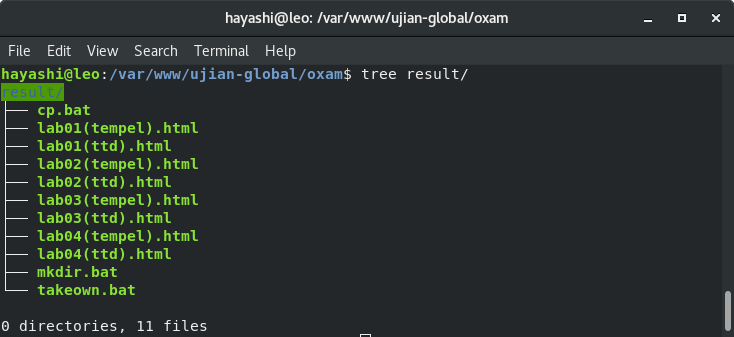
\includegraphics[width=0.7\paperwidth]{Gambar/ss-struktur-folder-generator.png}
    \caption{Daftar peserta yang di\textit{generate} oleh Oxam dalam bentuk
    berkas.}
    \label{fig:ss-folder-gen}
\end{figure}

Petugas Admin yang berkewajiban untuk menjaga harus memastikan bahwa kumpulan
berkas ujian yang lama harus dihapus terlebih dahulu sebelum memulai sesi ujian
yang baru. Jika petugas tersebut lupa, maka konsekuensinya adalah pada saat
pengumpulan, Admin yang bertugas harus memisahkan berkas ujian lama dan yang
baru secara manual.

Masalah berikutnya muncul pada saat proses ujian tersebut berjalan. Pertama,
terdapat \textit{bug} waktu ujian telah habis, pada kenyataannya waktu ujian
belum habis. Kedua, \textit{timer} yang digunakan untuk menunjukan sisa waktu
ujian tidak tersingkronisasi dengan Oxam. Sehingga pada saat timer berbunyi,
tempat pengumpulan tidak langsung tertutup. Ketiga, entri ujian yang sudah
dihapus masih muncul pada tempat pengumpulan. Hal ini biasanya Admin tangani
dengan cara mengubah tanggal sesinya ke tahun lalu.

Pada fase pengumpulan berkas jawaban ujian ke dosen koordinator, sistem tidak
secara otomatis mengumpulkan berkas tersebut. Sehingga seringkali Admin yang
bertugas lupa untuk mengirimkan berkas tersebut. Pengumpulan berkas tersebut
seharusnya dikirimkan sesegera mungkin saat ujian sudah selesai. Hal ini
dimaksudkan agar jawaban tidak diubah di kemudian hari tanpa izin.

Selain masalah-masalah pada tiap fase tersebut, masalah lain ada pada sistem itu
sendiri. Oxam menyimpan berkas tanpa mengacak lokasi atau nama berkas jawaban
tersebut, diperlihatkan pada Gambar \ref{fig:ss-folder-jawaban}. Hal ini dapat
mempermudah penyerang sistem untuk mengubah berkas jawaban tersebut.

\begin{figure}
    \centering
    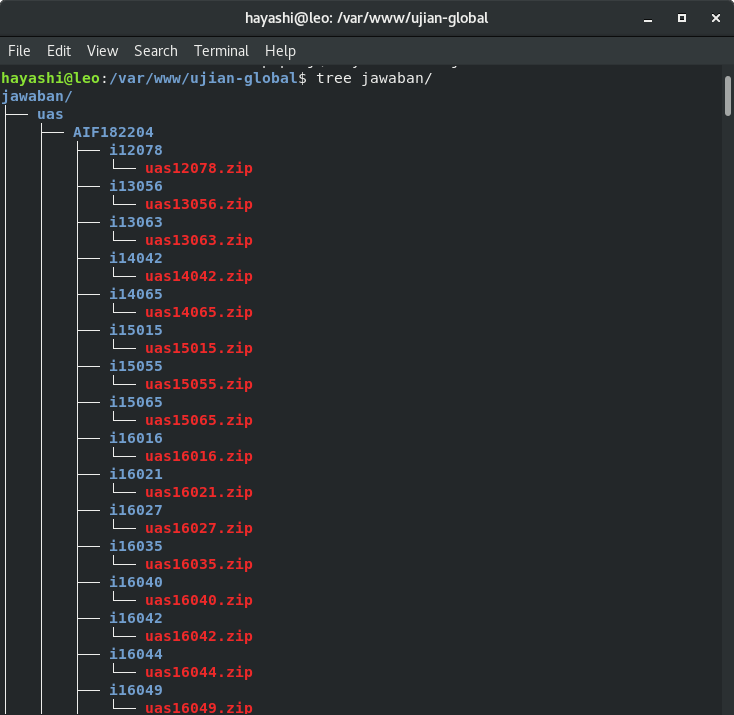
\includegraphics[width=0.6\paperwidth]{Gambar/ss-struktur-folder-jawaban.png}
    \caption{Struktur folder jawaban pada sistem Oxam.}
    \label{fig:ss-folder-jawaban}
\end{figure}

Pada penelitian ini, diharapkan akan menghasilkan perangkat lunak baru untuk
menyelesaikan masalah-masalah yang muncul pada perangkat lunak lama dengan
menggunakan \textit{framework Fat-free} dan \textit{React.js}.

\section{Rumusan Masalah}
\label{sec:rumusan}
Pada skripsi ini, aplikasi akan membantu memecahkan masalah:
\begin{itemize}
    \item Apa saja kebutuhan perangkat lunak untuk ujian untuk sistem manajemen
    ujian di lab komputasi?
    
    \item Bagaimana implementasi pemenuhan kebutuhan perangkat lunak sistem
    manajemen ujian di lab komputasi?
\end{itemize}

\section{Tujuan}
\label{sec:tujuan}
Tujuan dari skripsi ini adalah sebagai berikut:
\begin{itemize}
    \item Melakukan survei dan analisis untuk mendapatkan daftar kebutuhan
    perangkat lunak ujian untuk sistem informasi manajemen ujian di lab
    komputasi.
    \item Pemenuhan kebutuhan diimplementasi dengan membuat ulang perangkat
    lunak dengan menggunakan \textit{framework}, dengan harapan dapat terus di
    pelihara oleh tim admin di kemudian hari.
\end{itemize}

\section{Batasan Masalah}
\label{sec:batasan}
Batasan masalah pada penelitian ini adalah sebagai berikut:
\begin{enumerate}
    \item Solusi yang diajukan akan berupa aplikasi pendukung sistem ujian.
  
    \item Aplikasi pendukung ujian akan berjalan pada server berbasis Linux,
    sehingga dibutuhkannya bantuan untuk mengeksekusi \textit{script batch} pada
    sistem berbasis Windows.
\end{enumerate}

\section{Metodologi}
Metodologi yang dilakukan pada penelitian ini adalah sebagai berikut:
\label{sec:metlit}
    \begin{enumerate}
        \item Studi literatur bahasa dan \textit{framework} Fat-free dan
        \textit{libary} React.js.
        \item Melakukan survei sistem dan menyebar kuisioner.
		\item Melakukan perancangan ERD basis data.
		\item Melakukan perancangan tampilan antarmuka.
		\item Mengimplementasi modul/entitas berikut:
		    \begin{itemize}
		        \item Mata Kuliah
		        \item Peserta Ujian
		        \item Ujian (Sesi Ujian)
		        \item Print Daftar Peserta
		        \item Pengumuman untuk Peserta
		    \end{itemize}
	     \item Implementasi Tampilan untuk Peserta dengan detil:
		    \begin{itemize}
		        \item Tempat Pengumpulan
		        \item \textit{Sumary} Ujian
		        \item Bagian informasi/notifikasi
		    \end{itemize}
		\item Implementasi Admin Panel untuk Admin.
	    \item Melakukan \textit{deployment} dan pengujian pada fungsionalitas
	    perangkat lunak.
	    \item Implementasi pengiriman berkas jawaban ujian secara otomatis ke
	    dosen bersangkutan.
        \item Menarik kesimpulan dan saran berdasarkan proses penelitian dan
        pengujian.
    \end{enumerate}

\section{Sistematika Pembahasan}
\label{sec:sispem}

Pembahasan penelitian akan dilakukan secara sistematis dengan detail sebagai
berikut:

\begin{itemize}
    \item Bab 1 Pendahuluan \\
        Berisi latar belakang penelitian, rumusan masalah, tujuan batasan
        masalah, metodologi dan sistematika pembahasan penelitian.
    
    \item Bab 2 Landasan Teori \\
        Bab ini berisi teori dari Back-end dan Front-end, Framework, REST API,
        CI/CD dan Docker.
        
    \item Bab 3 Analisis \\
        Berisi pembahasan analisa sistem masa kini, pelaksanaan ujian,
        kuisioner, analisa kebutuhan dan fitur aplikasi, pemilihan
        \textit{framework} & \textit{library}, serta Analisis pengguna.
        
        
    \item Bab 4 Perancangan \\
        Berisi rancangan yang dibuat berdasarkan hasil analisis pada bab
        sebelumnya.
    
    \item Bab 5 Implementasi dan Pengujian \\
        Berisi pembahasan implementasi aplikasi yang dirancang dan pengujian
        aplikasi tersebut.
        
    \item Bab 6 Kesimpulan dan Saran \\
        Berisi kesimpulan dan saran dari penelitian ini.
\end{itemize}